\documentclass{article} % fonte 11 points, papier a4
\usepackage[francais]{babel}    % faire du français
\usepackage[utf8]{inputenc}   % accents dans le source
\usepackage[T1]{fontenc}        % accents dans le DVI
\usepackage{url}                % citer des adresses électroniques et des URL

\usepackage[total={6.5in,8.75in},top=1.1in, left=0.99in, right=0.99in]{geometry}

\geometry{hmargin=2.5cm,vmargin=2cm}

\usepackage{xcolor}
\usepackage{graphicx}
\usepackage{hyperref}
\hypersetup{
pdfborder={0 0 0 [3 3]},
pdftitle={{CV Adel Ferdjoukh}},
pdfauthor={Adel Ferdjoukh},
colorlinks=false
}

\newcommand{\nb}[2]{
    \fbox{\bfseries\sffamily\scriptsize#1}
    {\sf\small\textit{\textcolor{red}{#2}}}
}

\newcommand\ad[1]{\nb{Adel}{#1}}
\newcommand\adel[1]{\nb{Adel}{#1}}
\newcommand\Adel[1]{\nb{Adel}{#1}}

\usepackage{fancyhdr}
\pagestyle{fancy}
\renewcommand\headrulewidth{0pt}
\fancyhead{~}
\fancyfoot[C]{update \today}
\fancyfoot[L]{CV $-$ Adel Ferdjoukh}
\fancyfoot[R]{\thepage}
\def«{\og\ignorespaces}
\def»{{\fg}}

% For big titles
\newcommand{\mytitle}[1]{%
	%\rule{\textwidth}{.3pt}
	\par
  %\vspace{0.1cm}
   ~~\textbf{{#1}}
   \vspace{-2mm}
  
	\rule{\textwidth}{.3pt}
	}

%titles in left
\newcommand{\lefttitle}[1]{%
  \begin{flushleft}
  \mytitle{#1}
  \end{flushleft}
  %\bigskip
  }

%titles in right
\newcommand{\righttitle}[1]{%
  \begin{flushleft}
  \mytitle{#1}
  \end{flushleft}
  %\bigskip
  }

%Define notes
\newcommand{\note}[1]{
    \vspace{3mm}
    \rule{0.3\textwidth}{0.2mm}
    \par\vspace{1mm}
    {\bf Note:} #1}

\newcommand{\tair}{\vspace{3mm}}
\newcommand{\air}{\vspace{3mm}}
\newcommand{\oair}{\vspace{1mm}}


\newcommand{\fr}{
\includegraphics[scale=0.02]{img/fr.png}}
\newcommand{\dz}{
\includegraphics[scale=0.02]{img/dz.png}}
\newcommand{\kab}{
\includegraphics[scale=0.02]{img/kab.png}}

\newcommand{\web}{
\includegraphics[scale=0.15]{img/web.png}}
\newcommand{\email}{
\includegraphics[scale=0.15]{img/email.png}}
\newcommand{\phone}{
\includegraphics[scale=0.15]{img/phone.png}}

\newcommand{\grimm}{$\mathcal{G}$\textsc{rimm}}
\newcommand{\grimmtext}{$\mathcal{G}$ene\textsc{r}ating \textsc{i}nstances of \textsc{m}eta-\textsc{m}odels}
\DeclareRobustCommand{\grrimm}{$\mathcal{G}$\reflectbox{\textsc{r}}\textsc{rimm}}
\DeclareRobustCommand{\grrimmtext}{$\mathcal{G}$enerating \reflectbox{\textsc{r}}andomized and \textsc{r}elevant \textsc{i}nstances of \textsc{m}eta-\textsc{m}odels}
\newcommand{\comodi}{\textsc{comodi}}


%%%%%%%%%%%%%%%%%%%%%%%%%%%%%%%%%%%%%%
%                                    %
%  Biblio                            %
%                                    %
%%%%%%%%%%%%%%%%%%%%%%%%%%%%%%%%%%%%%%
\usepackage{natbib}
\usepackage{bibentry}
\bibliographystyle{plainnat}

\usepackage[object=vectorian]{pgfornament} %%  http://altermundus.com/pages/tkz/ornament/index.html

\usepackage{tikz}

\newcommand{\sectionline}{%
  \noindent
  \begin{center}
  {\color{black}
    \resizebox{0.5\linewidth}{1ex}
    {{%
    {\begin{tikzpicture}
    \node  (C) at (0,0) {};
    \node (D) at (9,0) {};
    \path (C) to [ornament=85] (D);
    \end{tikzpicture}}}}}%
    \end{center}
  }

\begin{document}

\thispagestyle{empty}

%%%%%%%%%%%%%%%%%%%%%%%%%%%%%%%%%%%%%%
%                                    %
%  TOP CV page FR                    %
%                                    %
%%%%%%%%%%%%%%%%%%%%%%%%%%%%%%%%%%%%%%
\thispagestyle{empty}

%Remove the biblio title
\renewcommand\refname{~}

\begin{center}
\par\textbf{\huge Curriculum Vitae}
\end{center}

\vspace{.5cm}

\begin{minipage}{0.45\textwidth}
\textbf{Adel Ferdjoukh, Dr.} \\ 
Vienne, Autriche

\vspace{.3cm}

Nationalités \fr{} \dz{} \kab{} \\
27 ans \\

\begin{tabular}{cl}
\email{} & ferdjoukh@gmail.com\\

\web{} & \url{http://adel-ferdjoukh.ovh}\\
\end{tabular}

\medskip
{\bf Spécialité}: Informatique, Génie Logiciel, Ingénierie Dirigée par les Modèles.

\medskip
{\bf Poste actuel}: Chercheur post-doctorant à TU Wien (Université Technique de Vienne).

%\medskip
%{\bf Référents}: Clémentine Nebut (nebut@lirmm.fr, co-directrice de thèse), Marianne Huchard (huchard@lirmm.fr, directrice de thèse).

\end{minipage}
\hfill
\begin{minipage}{0.45\textwidth}
\begin{flushright}
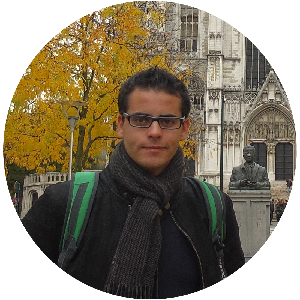
\includegraphics[scale=0.25]{img/me2.png}~~~~~~~~
\end{flushright}
\end{minipage}


\tair

\sectionline{}


%%%%%%%%%%%%%%%%%%%%%%%%%%%%%%%%%%%%%%%%%%%%%%%%%%%%%%%%%
%                                                       %
% Research experience                                   %    
%                                                       %
%%%%%%%%%%%%%%%%%%%%%%%%%%%%%%%%%%%%%%%%%%%%%%%%%%%%%%%%%
%%%%%%%%%%%%%%%%%%%%%%%%%%%%%%%%%%%%%%%%%%%%%%%%%%%%%%%%%
%                                                       %
% Work                                                  %    
%                                                       %
%%%%%%%%%%%%%%%%%%%%%%%%%%%%%%%%%%%%%%%%%%%%%%%%%%%%%%%%%
\righttitle{Expériences Professionnelles}

\begin{tabular}{r @{~$\rangle$~} p{0.85\textwidth}}
\oair

\textbf{2019 $\rightarrow$} & {\bf Software Architect, R\&D Project Leader} à Altran Technologies, Toulouse. \\
\oair

\textbf{2018} & {\bf Chercheur post-doctorant} à TU Wien, Autriche. Équipe de recherche: BIG. \\
\oair

\textbf{2016-2018} & {\bf Enseignant-chercheur non titulaire (ATER)} à l'Université de Nantes. Équipe de recherche: Atlanmodels. \\
\oair

\textbf{2014-2016} & {\bf Enseignant non titulaire (Mission complémentaire d'enseignement)} à l'Université de Montpellier. \\
\oair

\textbf{2013-2016} & \textbf{Doctorant} au Lirmm de Montpellier. Domaine de recherche: Model Based Engineering. \\
\oair

\textbf{2013} & \textbf{Stagiaire de recherche} au laboratoire Lirmm de Montpellier. \\

\end{tabular}


%%%%%%%%%%%%%%%%%%%%%%%%%%%%%%%%%%%%%%
%                                    %
%  Ens                               %
%                                    %
%%%%%%%%%%%%%%%%%%%%%%%%%%%%%%%%%%%%%%
%%%%%%%%%%%%%%%%%%%%%%%%%%%%%%%%%%%%%%
%                                    %
%  Projets                           %
%                                    %
%%%%%%%%%%%%%%%%%%%%%%%%%%%%%%%%%%%%%%
\lefttitle{Principaux projets}

\begin{tabular}{r @{~$\rangle$~} p{0.8\textwidth} l}

\textbf{HQ Workbench} & Software Architect, A Digital Transformation of HQ department (FD\&S initiative). Airbus \\

\textbf{IPad} & Technical Leader, A workbench for launching aerodynamics studies. Airbus \\

\textbf{Icing} & Développeur, New Approach for Icing Tools \& Data Management. Airbus \\

\textbf{Optimind} & R\&D Project Leader, a Model-Driven toolbox for engineers. Altran research \\

\textbf{RUMOR} & Développeur, Automate and migrate simulation tools. Airbus \\

\textbf{LEA$_{xDSML}$} & Exécution de transformations de modèles. Vienne, Autriche \\
 
\textbf{Tiwizi} & Debuggeur de modèles. Université de Nantes \\

\textbf{CoMoDi} & Comparateur de modèles. Université de Nantes \\

\textbf{Grimm} & Générateur automatique de modèles. Université de Montepllier \\

\end{tabular}

%%%%%%%%%%%%%%%%%%%%%%%%%%%%%%%%%%%%%%
%                                    %
%  Etudes                            %
%                                    %
%%%%%%%%%%%%%%%%%%%%%%%%%%%%%%%%%%%%%%
% %%%%%%%%%%%%%%%%%%%%%%%%%%%%%%%%%%%%%%%%%%%%%%%%%%%%%%%%%
%                                                       %
%    Study                                              %    
%                                                       %
%%%%%%%%%%%%%%%%%%%%%%%%%%%%%%%%%%%%%%%%%%%%%%%%%%%%%%%%%
\lefttitle{Études}

\begin{tabular}{r @{~$\rangle$~} p{0.8\textwidth}}
\oair

\textbf{2013-2016} & {\bf Thèse de doctorat en informatique} de l'Université de Montpellier, intitulée: "Approche déclarative pour la génération de modèles", soutenue le 20 octobre 2016 devant:

\begin{itemize}
    \item Présidente du jury: Carmen Gervet.
	\item Rapporteurs: Jean-Michel Bruel et Michel Rueher.
	\item Examinateur: Frank Barbier.
	\item Directrice et co-directrice: Marianne Huchard et Clémentine Nebut.
	\item Encadrants de thèse: Eric Bourreau et Annie Chateau.
\end{itemize}
\\

\oair

\textbf{2012-2013} & {\bf Master 2 en informatique (génie logiciel, programmation par contraintes)} à l'Université Montpellier 2 (Moyenne annuelle: 16/20, Major de promotion)

\begin{itemize}
    \item Stage de recherche intitulé: {\it Génération de modèles: une approche par modélisation CSP} et encadré par: Clémentine Nebut, Rémi Coletta, Anne-Élisabeth Baert et Annie Chateau.
\end{itemize}
 \\
\oair


\textbf{2011-2012} & {\bf Master 1 en réseaux et systèmes distribués} à l'Université de Bejaia en Algérie. (Moyenne annuelle: 14.84/20, Major de promotion). \\
\oair

\textbf{2009-2011} & {\bf Licence en Informatique} générale à l'Université de Bejaia sur la création de portails web avec la technologie .NET de Microsoft. (reçu $3^{ieme}/200$) \\

\textbf{Juin 2008} & {\bf Baccalauréat série Mathématiques} (Mention Assez bien) \\

\end{tabular}

\air
%%%%%%%%%%%%%%%%%%%%%%%%%%%%%%%%%%%%%%%%%%%%%%%%%%%%%%%%%
%                                                       %
%    Study                                              %    
%                                                       %
%%%%%%%%%%%%%%%%%%%%%%%%%%%%%%%%%%%%%%%%%%%%%%%%%%%%%%%%%
\lefttitle{Études}

\begin{tabular}{r @{~$\rangle$~} p{0.85\textwidth}}
\oair

\textbf{2016} & {\bf Thèse de doctorat en informatique} de l'Université de Montpellier, intitulée: ``Approche déclarative pour la génération de modèles''. \\
\oair

\textbf{2013} & {\bf Master 2 en informatique (génie logiciel, programmation par contraintes)} à l'Université Montpellier 2 \\
\oair

\textbf{2012} & {\bf Master 1 en réseaux et systèmes distribués} à l'Université de Bejaia en Algérie. \\
\oair

\textbf{2011} & {\bf Licence en Informatique} générale à l'Université de Bejaia sur la création de portails web avec la technologie .NET de Microsoft. \\
\oair

\textbf{2008} & {\bf Baccalauréat série Mathématiques} \\

\end{tabular}

\air

%%%%%%%%%%%%%%%%%%%%%%%%%%%%%%%%%%%%%%
%                                    %
%  notables                          %
%                                    %
%%%%%%%%%%%%%%%%%%%%%%%%%%%%%%%%%%%%%% 
\righttitle{Faits notables}

\begin{tabular}{r @{~$\rangle$~} p{0.55\textwidth}}
\oair
\textbf{Talks dans congrès ou rencontres} & Montpellier, Nantes, Lille, Angers, Paris, Bordeaux, Washington DC, San Francisco, Oslo, Copenhague, Athènes, Vienne. \\

\oair
\textbf{Enseignement et recherche} & Université de Montpellier, Université de Nantes, TU Wien (Autriche), Simula Lab (Norvège, Invité). \\

\oair
\textbf{Publications scientifiques} & 10 publications internationales. \\

\oair
\textbf{Industriels} & Airbus \\
\end{tabular}

%%%%%%%%%%%%%%%%%%%%%%%%%%%%%%%%%%%%%%%%%%%%%%%%%%%%%%%%%
%                                                       %
% Publication FR                                        %    
%                                                       %
%%%%%%%%%%%%%%%%%%%%%%%%%%%%%%%%%%%%%%%%%%%%%%%%%%%%%%%%%
%%%%%%%%%%%%%%%%%%%%%%%%%%%%%%%%%%%%%%%%%%%%%%%%%%%%%%%%%
%                                                       %
%    Publications                                       %    
%                                                       %
%%%%%%%%%%%%%%%%%%%%%%%%%%%%%%%%%%%%%%%%%%%%%%%%%%%%%%%%%
\lefttitle{Publications internationales}

\begin{tabular}{r @{~$\rangle$~} p{0.65\textwidth}}

Nombre de publications & $1$ article de revue internationale, $5$ articles en conférences internationales avec comités de lecture et actes, $1$ article en workshop international avec actes et comité de lecture et $1$ article (en Anglais) en conférence française avec actes\\
Taux d'acceptation & entre $27\%$ et $40\%$\\
Best Paper Award & ICSEA 2017 (Athènes, Grèce)\\
Total des citations & $50$ (au 25.08.2018)\\
\end{tabular}

% \nobibliography{biblio}

% \begin{itemize}
% \tair
% \item \bibentry{ferdjoukh17}
% \tair
% \item \bibentry{ferdjoukh13}
% \tair
% \item \bibentry{ferdjoukh15}
% \tair
% \item \bibentry{ferdjoukh16}
% \tair
% \item \bibentry{galinier16}
% \end{itemize}

%%%%%%%%%%%%%%%%%%%%%%%%%%%%%%%%%%%%%%
%                                    %
%  Ens                               %
%                                    %
%%%%%%%%%%%%%%%%%%%%%%%%%%%%%%%%%%%%%%
%%%%%%%%%%%%%%%%%%%%%%%%%%%%%%%%%%%%%%
%                                    %
%  Enseignement                      %
%                                    %
%%%%%%%%%%%%%%%%%%%%%%%%%%%%%%%%%%%%%%
\righttitle{Enseignement}

\begin{tabular}{r @{~$\rangle$~} p{0.7\textwidth}}

Universités & Univ. Montpellier (2 ans), Univ. Nantes (2 ans). \\
Matières enseignées & Algorithmique \& Programmation, Structures de données, programmation orientée Objet, Bases de données, Réseaux, Programmation Web, Ingénierie dirigée par les modèles et C2i, Développement logiciel, Programmation avancée  \\

Technologies et langages & C/C++, bash, Java, SQL, HTML/CSS, PHP, Javascript, Typescript, Git, Eclipse, EMF.\\

Cursus étudiants & Licence 1,2 \& 3. Master 1 \& 2. \\
Total des heures & $600$ heures. \\
\end{tabular}


%%%%%%%%%%%%%%%%%%%%%%%%%%%%%%%%%%%%%%
%                                    %
%  Encadrement                       %
%                                    %
%%%%%%%%%%%%%%%%%%%%%%%%%%%%%%%%%%%%%%
%%%%%%%%%%%%%%%%%%%%%%%%%%%%%%%%%%%%%%
%                                    %
%  Ecadrement                        %
%                                    %
%%%%%%%%%%%%%%%%%%%%%%%%%%%%%%%%%%%%%%
\lefttitle{Encadrement d'étudiants et de projets}

\begin{tabular}{r @{~$\rangle$~} p{0.8\textwidth} l}

\textbf{2013-2014} & Felix Vonthron et Olivier Perrier (stage d'été, Master 1) \tair \\

\textbf{2014-2015} & Florian Galinier (stage d'été, Master 1) \tair \\

\textbf{2015-2016} & Florian Galinier (stage de fin d'études, Master 2) \\
                   & Meddy Urie (stage de fin d'études, IUT)\\
                   & Timothee Martinod et Florian Novellon (stage d'été, Licence 2) \\

\end{tabular}

%%%%%%%%%%%%%%%%%%%%%%%%%%%%%%%%%%%%%%
%                                    %
%  Recherche divers                  %
%                                    %
%%%%%%%%%%%%%%%%%%%%%%%%%%%%%%%%%%%%%%
\lefttitle{Participation à la communauté scientifique}

\begin{tabular}{r @{~$\rangle$~} p{0.75\textwidth}}

{\bf Chercheur visiteur} & laboratoire Simula, Oslo, mars 2017. \\

{\bf Collaboration} & Implication dans un projet européen d'échange entre l'équipe Atlandmodels à Nantes et Simula à Oslo (Dizolo, 2017) \\

{\bf Rapporteur} & JFPC'14, MODELSWARD'16, ISSRE'17, ICWE'18, RCIS'18, ICSEA'18 \\

{\bf Volontariat} & ECOOP/ECSA/ECMFA'13 \\

{\bf Autre} & École d'été ACAI'15. \\

\end{tabular}

%%%%%%%%%%%%%%%%%%%%%%%%%%%%%%%%%%%%%%
%                                    %
%  Vie associative                   %
%                                    %
%%%%%%%%%%%%%%%%%%%%%%%%%%%%%%%%%%%%%%
%%%%%%%%%%%%%%%%%%%%%%%%%%%%%%%%%%%%%%
%                                    %
%  Vie associative                   %
%                                    %
%%%%%%%%%%%%%%%%%%%%%%%%%%%%%%%%%%%%%%
\righttitle{Vie associative et volontariat}

\begin{tabular}{r @{~$\rangle$~} p{0.85\textwidth}}
\oair
{\bf 16-18} & {\bf Webmaster et infographiste} de l'association culturelle berbère de Loire-Atlantique ({\it voir www.berberes44.fr}). \\

\oair

{\bf 14-15} & {\bf Co-organisation} des séminaires des doctorants du laboratoire lirmm (Semindoc@Lirmm). \\
\oair

{\bf 01-06/14} & {\bf Co-organisation} de la journée de conférences des doctorants de Montpellier (Doctiss'14). \\
\oair

{\bf 06/13} & {\bf Étudiant Volontaire} aux conférences Ecoop, Ecsa, Ecmfa, Montpellier, France. \\
\oair

\textbf{11-12} & \textbf{Président d'un club scientifique informatique} d'étudiants au sein de l'Université de Bejaia. \\
\oair

\textbf{2012} & \textbf{Chargé de la Communication} de l'association de la sauvegarde du patrimoine de la ville de Bejaia en Algérie.   \\

\end{tabular}

%%%%%%%%%%%%%%%%%%%%%%%%%%%%%%%%%%%%%%%%%%%%%%%%%%%%%%%%%
%                                                       %
%        Bourses                                        %    
%                                                       %
%%%%%%%%%%%%%%%%%%%%%%%%%%%%%%%%%%%%%%%%%%%%%%%%%%%%%%%%%
\righttitle{Bourses et récompenses}

\begin{tabular}{r @{~$\rangle$~} p{0.8\textwidth} l}
\oair
{\bf 2017} & <<Best Paper Award>> à la conférence ICSEA à Ahtène, Grèce. \\
\oair
{\bf 2013} & Allocation de recherche sur concours doctoral de l'école doctorale I2S de Montpellier. \\
\oair
{\bf 2012} & Bourse d'excellence européenne de mobilité ({\it programme Averroés}). \\
\end{tabular}

%%%%%%%%%%%%%%%%%%%%%%%%%%%%%%%%%%%%%%
%                                    %
%  Langues                           %
%                                    %
%%%%%%%%%%%%%%%%%%%%%%%%%%%%%%%%%%%%%%
%%%%%%%%%%%%%%%%%%%%%%%%%%%%%%%%%%%%%%
%                                    %
%  Langues                           %
%                                    %
%%%%%%%%%%%%%%%%%%%%%%%%%%%%%%%%%%%%%%
\lefttitle{Langues pratiquées}


Français, Anglais, Arabe, Kabyle, Allemand (débutant)

	


%%%%%%%%%%%%%%%%%%%%%%%%%%%%%%%%%%%%%%
%                                    %
%  Compétences informatiques         %
%                                    %
%%%%%%%%%%%%%%%%%%%%%%%%%%%%%%%%%%%%%%
%%%%%%%%%%%%%%%%%%%%%%%%%%%%%%%%%%%%%%
%                                    %
%  Compétences informatiques         %
%                                    %
%%%%%%%%%%%%%%%%%%%%%%%%%%%%%%%%%%%%%%
\righttitle{Compétences informatiques}

\begin{tabular}{r @{~$\rangle$~} p{0.7\textwidth} l}
\oair

\textbf{Avancé à Expert} & Java, EMF, Eclipse, RCP, Bash, C, R, HTML/CSS, SQL, Javascript, PHP, \LaTeX \\
\oair

\textbf{Notions à Moyen} & C++, Python, programmation par contraintes, ASP.NET, Pascal, programmation réseaux, Matlab, Prolog \\
\end{tabular}

\end{document}